% -------------------------------------------------------
% Challenge: AAPG Generation Test
% -------------------------------------------------------
\section{Challenge 2 Level 2 (C2L2): AAPG Generation Test}

In this Section, Challenge 2 Level 2 (C2L2) is presented. First, a description of the challenge is explained, second, the implementation to solve is presented, and finally, a discussion about the AAP tool is given. 

\subsection{Description}

The challenge is to create an AAPG (Automated Assembly Program Generator) config file that generates a test with 10 illegal exceptions, each with the correct handler code. This challenge aims to assess the ability to configure the AAPG tool to produce specific test cases with the desired number of illegal exceptions and their corresponding handlers.

\subsection{Solution}

To complete this challenge, the following steps were followed:

\begin{enumerate}
    \item The config file used in ``challenge\_level2/challenge\_instructions" was copied to this directory. The existing config file likely specified configurations for the RV32I base integer instruction set and other relevant parameters.
    \item The line in ``rv32i.yaml" was updated from:
    
\begin{minted}[frame=single]{nasm}
ecause02: 0
\end{minted}

    to:
    
\begin{minted}[frame=single]{nasm}
ecause02: 9
\end{minted}
    
    This modification sets the value of \texttt{ecause02} to 9, effectively instructing the AAPG to generate 10 illegal exceptions during the test.
    
    \item The AAPG tool was run to generate the assembly code based on the updated config file. The generated assembly code will contain the specified test cases with the desired illegal exceptions.
\end{enumerate}

The reason for using ``9" instead of "10" was due to the output log test, as shown in Figure \ref{fig:output_simulation}. Using ``9" resulted in 10 exceptions, in accordance with the challenge specification. 

\begin{figure}[h]
  \centering
  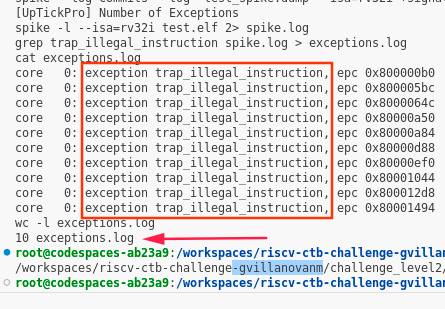
\includegraphics[width=0.47\textwidth]{./c2l2_img/img1.png}
  \caption{Output of the C2L2 simulation.}
  \label{fig:output_simulation}
\end{figure}

\subsection{How Is Exception Generated in AAPG?}

Configuring the \texttt{ecause02} fields and running AAPG will generate random assembly routines with exceptions. These routines are then incorporated into the \texttt{test.S} code, as shown in the figure below.

\begin{figure}[h]
  \centering
  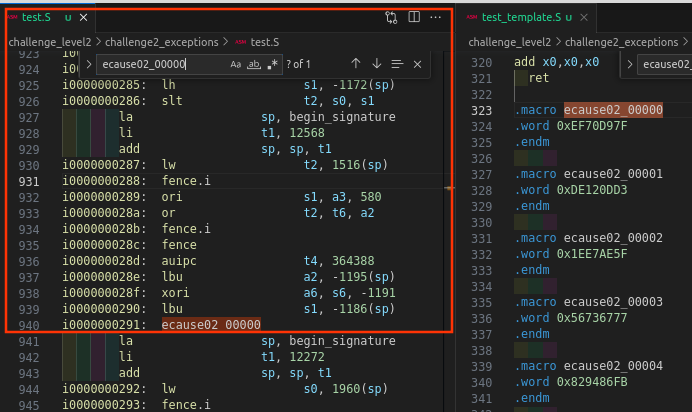
\includegraphics[width=1\linewidth]{./c2l2_img/expl.png}
  \caption{Code Generation Process}
\end{figure}

Each snippet will consist of a \texttt{.word} instruction, encompassing anything that does not meet the criteria for a legal instruction in the context of the system. This will cause an exception to be invoked.

This process resembles the challenge exercise found in \texttt{challenge\_level1/challenge3\_illegal}, where scenarios involving illegal instructions were encountered.

\subsection{AAPG Future Work}

When executing the config file presented in the last section, the output was not always the same. Sometimes, after execution, the simulation never stopped, and other times, the simulation stopped and returned the log presented in the last section.

Attempts were made to create some modifications in ``rv32i.yaml," but the same behavior persisted. It is suspected that there may be a bug in AAPG that causes this inconsistent behavior. Further investigation is needed to resolve this issue.

The inconsistent behavior observed during the AAPG execution raises concerns about the tool's reliability. It is crucial to investigate and address this issue to ensure consistent and accurate generation of assembly programs for testing and verification purposes.
